\begin{center}
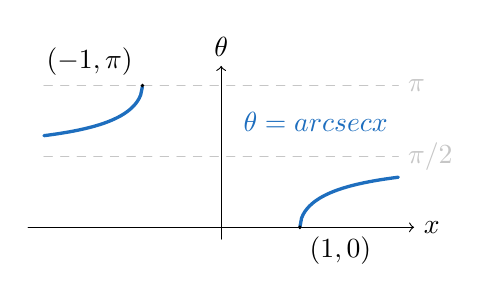
\begin{tikzpicture}[scale=1.0, line cap=round, line join=round]
  \definecolor{trigblue}{RGB}{30,110,190}
  \draw[->] (-2.45,0)--(2.45,0) node[right] {$x$};
  \draw[->] (0,-0.15)--(0,2.05) node[above] {$\theta$};
  \draw[gray!45,dashed] (-2.25,1.8)--(2.25,1.8) node[right] {$\pi$};
  \draw[gray!45,dashed] (-2.25,0.9)--(2.25,0.9) node[right] {$\pi/2$};
  \draw[very thick,trigblue,domain=1:2.25,samples=60]
    plot ({\x},{1.8*acos(1/\x)/180});
  \draw[very thick,trigblue,domain=-2.25:-1,samples=60]
    plot ({\x},{1.8*acos(1/\x)/180});
  \fill (1,0) circle (0.025) node[below right] {$(1,0)$};
  \fill (-1,1.8) circle (0.025) node[above left] {$(-1,\pi)$};
  \node[trigblue] at (1.2,1.34) {$\theta=\operatorname{arcsec} x$};
\end{tikzpicture}
\end{center}


\begin{definitionbox}{Definition}
\begin{definition}[Inverse secant]
\label{def:inverse-secant}
The \emph{inverse secant} function is the inverse of secant after secant is
restricted to $[0,\pi]\setminus\{\pi/2\}$. It is denoted by $\operatorname{arcsec}$ or
$\sec^{-1}$ and has domain $(-\infty,-1]\cup[1,\infty)$ and range
$[0,\pi]\setminus\{\pi/2\}$.
\[
  \operatorname{arcsec} x=\theta
  \quad\Longleftrightarrow\quad
  \sec\theta=x
  \quad\text{and}\quad
  0\leq\theta\leq\pi,\ \theta\neq\frac{\pi}{2}.
\]
\end{definition}
\end{definitionbox}
\begin{remark*}[Domain and range]
The secant function has domain
$\mathbb{R}\setminus\{\pi/2+k\pi:k\in\mathbb{Z}\}$ and range
$(-\infty,-1]\cup[1,\infty)$. The inverse secant function reverses the
principal restricted secant function.
\end{remark*}
\begin{dependencies}
\begin{itemize}
  \item \hyperref[def:extended-secant]{Extended secant}
  \item \hyperref[def:radian-measure]{Radian measure}
\end{itemize}
\end{dependencies}

\begin{theorembox}{Theorem}
\begin{theorem}[Principal inverse secant identities]
\label{thm:inverse-secant-identities}
For every $x\in(-\infty,-1]\cup[1,\infty)$,
\[
  \sec(\operatorname{arcsec} x)=x.
\]
For every $\theta\in[0,\pi]\setminus\{\pi/2\}$,
\[
  \operatorname{arcsec}(\sec\theta)=\theta.
\]
\end{theorem}
\end{theorembox}
\begin{remark*}[Standard quantified statement]
$\forall x\in(-\infty,-1]\cup[1,\infty)$, $\sec(\operatorname{arcsec} x)=x$, and
$\forall \theta\in[0,\pi]\setminus\{\pi/2\}$, $\operatorname{arcsec}(\sec\theta)=\theta$.
\end{remark*}
\begin{dependencies}
\begin{itemize}
  \item \hyperref[def:inverse-secant]{Inverse secant}
\end{itemize}
\end{dependencies}
